\documentclass[conference]{IEEEtran}
\usepackage{cite}
\usepackage{amsmath,amssymb}
\usepackage{graphicx}
\usepackage{booktabs}
\usepackage{textcomp}
\usepackage[hidelinks]{hyperref}
\usepackage{balance}
\IEEEoverridecommandlockouts
\renewcommand{\IEEEbibitemsep}{0pt plus 0.5pt}
\hyphenation{mini-chess Stock-fish}

\begin{document}

\title{Learning to Play Gardner Minichess: A Compute-Matched Comparison of Search, Evolutionary and Reinforcement-Learning Agents}

\author{\IEEEauthorblockN{Tanish Shitanshu}
\IEEEauthorblockA{Dept.\ of Computer Science and Engineering, Shiv Nadar University\\
CSD311 Artificial Intelligence, ts260@snu.edu.in}}

\maketitle

\begin{abstract}
We compare five techniques for Gardner $5\times5$ minichess, a game that is a proven draw: alpha-beta search with a hand-crafted evaluation, UCT Monte-Carlo tree search, the same search with an evaluation learned by TDLeaf($\lambda$) self-play (reinforcement learning), the same search with an evaluation evolved by a genetic algorithm (GA), and an AlphaZero-style network trained by self-play (reinforcement learning). All agents run on one C++ engine validated against Fairy-Stockfish and are compared at equal compute. At 400 nodes or simulations per move, the hand-crafted, TDLeaf and GA evaluations are within 47 Elo of each other, far above UCT MCTS ($-$598) and above the AlphaZero-style agent ($-$90, 95\% interval [$-$123, $-$63]). Starting from equal piece values and using only game results, TDLeaf gains +272 Elo; the GA reaches the same level from random weights. One simulation of the network agent costs about 12 alpha-beta nodes, and at equal wall-clock time it scores 0.25 against alpha-beta. The ranking agrees with play against Fairy-Stockfish at fixed depths and with per-move evaluation loss. An earlier version of our harness let both sides share one transposition table; the external checks exposed it, and we report what it had distorted. Code, data and an interactive board are released.

\end{abstract}

\begin{IEEEkeywords}
minichess, game-tree search, Monte-Carlo tree search, temporal-difference learning, genetic algorithm, AlphaZero, evaluation
\end{IEEEkeywords}

\section{Introduction}
Minichess has a long history, from the $6\times6$ program of Kister et al. \cite{kister1957}, and its variants are small enough to study complete learning pipelines on a laptop, yet they keep the structure that makes chess hard: tactics, king safety and a large gap between a naive and a good evaluation function. We use Gardner's $5\times5$ minichess (pieces \texttt{RNBQK}/\texttt{PPPPP}; no castling, double pawn step or en passant), which Mhalla and Prost showed to be a draw under perfect play \cite{mhalla2013}. Because the game-theoretic value is known, a strong agent should draw most games, and any win is a sign that the opponent has made a mistake.

We ask three questions. \textbf{RQ1:} which of five techniques is strongest when all are given the same compute budget? \textbf{RQ2:} what does learning add over hand-written knowledge, and where exactly is reinforcement learning (RL) used? \textbf{RQ3:} do wins against our own agents reflect real playing strength, or only the ability to exploit them? To answer RQ3 we use an independent engine, Fairy-Stockfish \cite{fairy}, as an external yardstick.

\textbf{Contributions.} (i) A C++ rules engine checked against Fairy-Stockfish move counts (perft) and wrapped for Python. (ii) Five agents sharing one engine: alpha-beta with a hand-crafted evaluation, UCT Monte-Carlo tree search (MCTS), an alpha-beta evaluation learned by TDLeaf($\lambda$) self-play, the same evaluation tuned by a genetic algorithm (GA), and an AlphaZero-style network trained by self-play. (iii) A compute-matched protocol: equal node or simulation budget, fixed openings, Bradley--Terry Elo with bootstrap intervals, an external Elo anchor and a per-move evaluation-loss measure. (iv) An interactive web platform and all code, so every number can be regenerated.

\section{Background}
Computer chess rests on minimax search with alpha-beta pruning \cite{shannon1950,knuth1975} and a heuristic evaluation. Samuel's checkers program already learned evaluation weights from play \cite{samuel1959}; temporal-difference (TD) learning produced TD-Gammon \cite{tesauro1995}, and TDLeaf($\lambda$) adapted TD learning to search-based programs such as chess \cite{baxter2000}. Monte-Carlo tree search with the UCT rule \cite{kocsis2006,coulom2007,browne2012} needs no evaluation function, only rollouts. AlphaZero \cite{silver2018,silver2017} replaced both with a neural network trained from self-play alone. Minichess has been used with such methods before \cite{sun2021,hammersborg2022}, and Pgx \cite{koyamada2023} provides GPU simulators; we instead keep a transparent, CPU-only pipeline and focus on a controlled comparison and on the quality of individual moves. Textbook background is in \cite{sutton2018,russell2021}.

\section{Methods}
\subsection{Game, engine and search budget}
The board is 25 squares; a move is a (from, to, promotion) triple. The engine implements legal-move generation, checkmate, stalemate, the 50-move rule, insufficient material and threefold repetition. Perft counts from the start position agree with Fairy-Stockfish's \texttt{gardner} variant to the depths we tested, and the unit tests (\texttt{pytest}) reproduce them. All agents are measured in the same currency, a \emph{budget} per move: alpha-beta counts visited nodes, MCTS and the AlphaZero-style agent count simulations. Our main budget is $B=400$.

\subsection{Alpha-beta with a linear evaluation}
The search is iterative-deepening negamax with alpha-beta pruning, a Zobrist-hashed \cite{zobrist1970} transposition table, killer and history heuristics, MVV-LVA capture ordering, quiescence search and a check extension; it stops when the node budget is used. Leaf positions are scored by a linear function of 14 features,
\begin{equation}
V(s)=\sum_{i=1}^{14} w_i\,\phi_i(s),
\end{equation}
seen from White. The features are: the White-minus-Black count of pawns, knights, bishops, rooks and queens; the number of pawns on the 3rd and on the 4th rank (relative to the owner); a centrality score for each of N, B, R, Q, K; the mobility of N, B, R, Q; and the number of friendly pieces adjacent to the king. The \emph{hand-crafted} weights are the textbook values 100/300/320/500/900 for material and small positional bonuses. Three agents share this search and differ only in $\mathbf{w}$: hand-crafted, TDLeaf-learned and GA-evolved.

\subsection{UCT Monte-Carlo tree search}
At a tree node with $N$ visits, the child $a$ with $n_a$ visits and mean value $Q_a$ maximises $Q_a + c\sqrt{\ln N / n_a}$ (we use $c=0.7$). A leaf is expanded and scored by a random rollout of at most 40 plies; if the game has not ended, the position is scored by a soft material count instead of being called a draw. The move with most visits is played.

\subsection{TDLeaf($\lambda$): reinforcement learning of the evaluation}
\textbf{Where RL is applied.} The state is the board, the action is the move returned by a depth-3 alpha-beta search (with probability $\epsilon=0.15$ a random legal move is played for exploration), and the only reward is the final result $z\in\{+1,0,-1\}$ from White's view. The value function is $V(s)=\tanh(\mathbf{w}\cdot\boldsymbol\phi(s)/400)$. Because the program plays the move found by search, the TD update uses the value of the principal-variation leaf $l_t$ of each search rather than of the root position \cite{baxter2000}. With $d_t=V(l_{t+1})-V(l_t)$ and $V(l_T):=z$,
\begin{equation}
\Delta\mathbf{w}=\alpha\sum_{t}\nabla_{\mathbf{w}}V(l_t)\sum_{j\ge t}\lambda^{\,j-t}d_j .
\end{equation}
In words: each leaf value is nudged towards the values that follow it, and the final result is passed back to earlier positions with decay $\lambda=0.7$. Weights start with all five piece types equal to 100 and all positional weights zero, so no chess knowledge is given. We train on 8000 self-play games, normalising each coordinate of the step by the running RMS of its feature.

\subsection{Genetic algorithm (evolution, not RL)}
A genome is the 14-vector $\mathbf{w}$. The population (32 genomes) is evaluated by playing each genome against randomly chosen others at budget 400 from random openings; fitness is the mean score. Selection is by 3-way tournament, recombination is blend crossover (BLX-0.3), mutation is Gaussian with decaying strength, and the two best genomes survive unchanged (elitism). Fitness is relative to the current population, so this is \emph{co-evolution} \cite{rosin1997}. We run two variants: unconstrained, and constrained by box limits that encode basic knowledge (every piece is worth at least 1.5 pawns, mobility is never negative). No gradient or per-move credit assignment is used, which is why this is not RL.

\subsection{AlphaZero-style self-play RL}
\textbf{Where RL is applied.} The state is the board as 12 one-hot piece planes seen from the side to move; the action is a (from, to) pair (625 outputs, illegal ones masked); the reward is the game result for the side to move. The network is a multilayer perceptron, $300\to H\to H$ with ReLU units, then a 625-way policy head and a tanh value head ($H=192$). Search is PUCT \cite{silver2018}: the child maximising
\begin{equation}
Q_a + c_{\text{puct}}\,P_a\,\frac{\sqrt{N}}{1+n_a},\qquad c_{\text{puct}}=1.5,
\end{equation}
where $P_a$ is the policy prior; Dirichlet noise ($\alpha=0.3$, weight $0.25$) is mixed into the root prior during self-play and the first 12 moves are sampled in proportion to visit counts. Each iteration plays 64 self-play games (the first move is random with probability one half to diversify games) with 150 simulations per move, stores (position, visit distribution $\boldsymbol\pi$, outcome $z$), and takes 120 Adam steps \cite{kingma2015} on random minibatches of the replay buffer to minimise
\begin{equation}
\mathcal{L}=(z-v)^2-\sum_a \pi_a\log p_a+c\,\lVert\theta\rVert^2 .
\end{equation}
Search turns the current network into a stronger policy (policy improvement); regressing onto the game result evaluates it; repeating both is policy iteration. Tree search, network inference and self-play run in C++; back-propagation is implemented in NumPy and its gradients were verified against finite differences.

\section{Experimental protocol}
All experiments use two CPU cores and no GPU. Every pairing is played from 60 fixed random openings of 2--4 plies, once with each colour (120 games); the same set is used for every pairing, so agents are not compared on different positions. Strength is reported as Elo from a Bradley--Terry maximum-likelihood fit \cite{bradley1952} with 95\% bootstrap intervals over games, anchored at the hand-crafted agent. \textbf{E1} is the round robin at $B=400$. \textbf{E2} plays each agent against Fairy-Stockfish at fixed depths 1--12 (20 openings, both colours). \textbf{E3} re-tests every saved checkpoint of every learner against the hand-crafted agent with the same protocol. \textbf{E4} measures move quality: for 300 positions reached by random play, we compare each agent's chosen move with Fairy-Stockfish's depth-9 evaluation and record the centipawn loss (the evaluation of the best line minus the evaluation after the agent's move, capped at 1000). A \emph{blunder} is a loss of at least 200 centipawns. We also measure how Elo scales with budget from 25 to 1600 and the wall-clock time per move.

\section{Results}
\begin{figure*}[t]
\centering
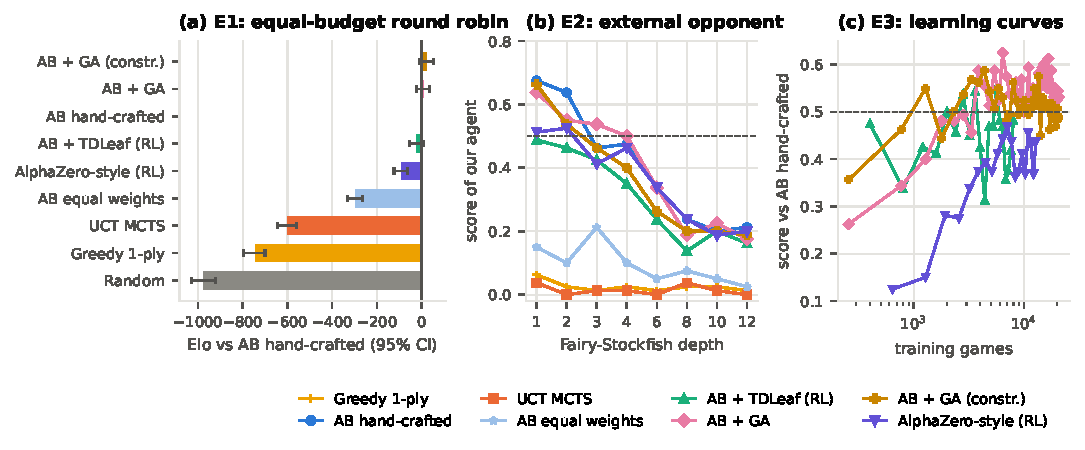
\includegraphics[width=\textwidth]{fig_report_a.pdf}
\caption{(a) Elo of every agent at an equal budget of 400 nodes or simulations, relative to the hand-crafted alpha-beta agent (bars: Bradley--Terry fit, whiskers: 95\% bootstrap interval; 120 games per pairing). (b) Score against Fairy-Stockfish at fixed depth (40 games per point; 0.5 = parity). (c) Score of each saved training checkpoint against the hand-crafted agent (same protocol).}
\label{fig:a}
\end{figure*}

\begin{table}[t]
\caption{Equal-budget results ($B=400$). Elo from the round robin; score against the hand-crafted agent; time per move; mean evaluation loss and blunder rate (loss $\ge200$ cp) from E4 (300 positions).}
\label{tab:main}
\centering
\small
\setlength{\tabcolsep}{3pt}
\resizebox{\columnwidth}{!}{%
\begin{tabular}{lcccrr}
\toprule
Agent & Elo [95\% CI] & vs hand & ms/move & loss (cp) & blund. \\
\midrule
Alpha-beta + GA (constr.) & +23 [-10, +53] & 0.53 & 0.2 & 61 & 9\% \\
Alpha-beta + GA & +7 [-24, +37] & 0.53 & 0.19 & 66 & 10\% \\
Alpha-beta, hand-crafted & +0 [+0, +0] & -- & 0.19 & 73 & 11\% \\
Alpha-beta + TDLeaf (RL) & -24 [-54, +7] & 0.44 & 0.2 & 83 & 13\% \\
AlphaZero-style (RL) & -90 [-123, -63] & 0.43 & 2.3 & 143 & 21\% \\
Alpha-beta, equal weights & -296 [-333, -265] & 0.13 & 0.2 & 125 & 19\% \\
UCT MCTS & -598 [-643, -558] & 0.02 & 5.7 & 386 & 50\% \\
Greedy 1-ply & -744 [-797, -700] & 0.01 & 0.013 & 260 & 34\% \\
Random & -973 [-1029, -921] & 0.00 & 0.009 & 612 & 71\%
\\
\bottomrule
\end{tabular}}
\end{table}

\textbf{E1, equal budget.} The four alpha-beta agents with a sensible evaluation (hand-crafted, TDLeaf, GA, constrained GA) are within 47 Elo of each other and their intervals overlap (about $\pm$32 Elo), so we cannot rank them. The AlphaZero-style agent is $-$90 Elo below the hand-crafted agent (95\% interval $-$123 to $-$63; score 0.43 against it, W28 D47 L45), the equal-weight agent is $-$296, and UCT MCTS is $-$598. TDLeaf starts from equal piece values and no positional knowledge, which is the equal-weight agent; the \emph{learned} weights are worth +272 Elo more. The GA, which starts from random weights, ends at +7 (unconstrained) and +23 (constrained).

\textbf{Cost.} A simulation of the network agent is much more expensive than an alpha-beta node: 2.3 ms against 0.19 ms per move at $B=400$. When alpha-beta is given the 6\,300 nodes it can search in the same time, the network agent scores only 0.25 against it (W12 D36 L72); at that budget alpha-beta reaches depth 4.0 instead of 1.8. UCT MCTS needs 5.7 ms per move and still scores 0.00 against time-matched alpha-beta.

\textbf{E2, external opponent.} (Fig.~\ref{fig:a}b.) The hand-crafted, GA and constrained-GA agents score 0.54--0.68 against Fairy-Stockfish at depths 1--2, hold roughly parity at depths 3--4 and score about 0.17--0.23 at depths 10--12. The AlphaZero-style and TDLeaf agents follow the same curve somewhat lower at shallow depth. The equal-weight agent averages 0.14 over depths 1--4 and the TDLeaf agent trained from it 0.43 (hand-crafted: 0.56); MCTS and the greedy agent score at most 0.06 even at depth 1.

\textbf{E3, learning curves.} (Fig.~\ref{fig:a}c.) All three learners start far below the hand-crafted agent and climb towards it. TDLeaf goes from 0.06 (equal weights) to about 0.45 within roughly 2400 games and then fluctuates; the GA climbs from 0.26 to about 0.55 within 4000 fitness games; the network agent rises from 0.12 to about 0.41 after roughly 7000 self-play games and then stays flat (policy loss 1.37). None settles above about 0.6.

\textbf{E4, move quality.} (Table~\ref{tab:main}.) The constrained GA, GA and hand-crafted agents lose 61, 66 and 73 cp per move and TDLeaf 83; their paired differences from the hand-crafted agent have bootstrap intervals that include zero. The equal-weight agent loses 125 cp and the AlphaZero-style agent 143 cp (70 cp more than hand-crafted, 95\% interval 36 to 103); its blunder rate is 21\% against 11\%.

\textbf{Learned weights and scaling.} (Fig.~\ref{fig:b}.) TDLeaf values knight, bishop, rook and queen at 2.4, 2.2, 3.8 and 4.9 pawns (hand-crafted: 3, 3.2, 5, 9); the unconstrained GA at 1.4, 1.3, 1.9 and 2.6. The order is right but the scale is compressed. Strength grows with budget for every agent: the network agent gains from $-$199 to +70 Elo between 25 and 1600 simulations (measured against alpha-beta at 400 nodes), and alpha-beta with the GA weights reaches 0.78 points at 1600 nodes; MCTS stays below 0.07 points against that opponent and is omitted from the plot.

\begin{figure*}[t]
\centering
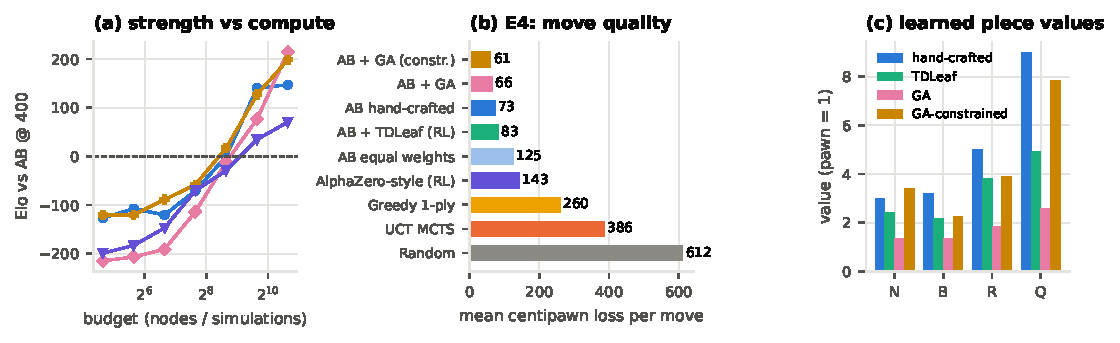
\includegraphics[width=\textwidth]{fig_report_b.pdf}
\caption{(a) Score-derived Elo against alpha-beta at 400 nodes as a function of budget (60 games per point; UCT MCTS stays below $-400$ and is omitted). (b) Mean centipawn loss per move against Fairy-Stockfish depth 9 on 300 positions. (c) Piece values learned by TDLeaf and by the two genetic algorithms, relative to the pawn.}
\label{fig:b}
\end{figure*}

\section{Discussion}
\textbf{Learning recovers, but does not exceed, expert knowledge.} Two methods that were given no chess knowledge end close to a hand-written evaluation: the GA, from game scores inside its population, and TDLeaf, from the result signal (somewhat lower than the hand-crafted agent against the outside engine at shallow depth); the network agent, trained on search statistics, ends further behind. The GA and TDLeaf match the hand-crafted agent in move quality (E4). The learned piece values are smaller than the textbook ones. The GA tuned its weights at 400 nodes, where alpha-beta reaches depth about 1.8 (mean over our E4 positions), so part of what they encode may be a correction for shallow search; TDLeaf trained with depth-3 search. We did not test this, or the effect of board size.

\textbf{Why the AlphaZero-style agent is behind.} With 12\,800 games and a 216\,000-parameter perceptron, the network is a weaker evaluator than 14 hand-chosen features combined with exact tactics from quiescence search; its losses stop decreasing early, which suggests a limit of data or capacity rather than of training time, but we did not vary either. Its scaling curve is the steepest, so it is not hopeless, but each simulation costs about 12 nodes. The result should not be read as a statement about AlphaZero at scale.

\textbf{UCT MCTS} is limited by random rollouts: in a tactical game a single blunder decides the result, so value estimates are noisy and our budgets are small.

\textbf{A validity lesson.} In an earlier version of the harness both sides of a game shared one transposition table, so an agent could reuse scores computed with the other agent's weights. In that version the unconstrained GA scored 0.74 against the hand-crafted agent at 2000 nodes (now 0.48), and the AlphaZero-style agent looked like the strongest one. The inconsistency showed up only against Fairy-Stockfish: an agent that beat the hand-crafted one head to head scored near zero from depth 4. Each side now owns its table, and every number here was produced after the fix. Without an external opponent we might not have seen it.

\section{Inference}
The evidence supports: (1) game results alone are enough for TDLeaf to move an equal-weight evaluation by +272 Elo to hand-crafted level, and a GA reaches the same level from random weights; no learner is shown to be better than the hand-written weights, since all intervals overlap; (2) at this data and compute scale a search with a linear evaluation beats a small self-play network both at equal budget and at equal time, and UCT with random rollouts is far weaker; (3) the in-pool ranking agrees with an independent engine and with move-level analysis, which is why we trust it. It does not support: differences smaller than about $\pm$32 Elo; claims about seeds, since each learner was trained once; claims about larger networks, longer training, or other variants. The E4 positions and Fairy-Stockfish depth are proxies, not a calibrated Elo.

\section{Conclusion}
We compared five techniques for Gardner minichess on one engine under one compute currency. With the same alpha-beta search, an evaluation learned by TDLeaf or evolved by a GA from no knowledge reaches the level of a hand-written one; an AlphaZero-style network trained for 35 CPU-minutes does not, and costs more per simulation; random-rollout MCTS is far behind. External play against Fairy-Stockfish was essential to detect a harness error. Next steps are repeated seeds with confidence bands, GA fitness that includes an outside opponent or a hall of fame \cite{rosin1997}, convolutional networks with search-value targets, and the Silverman $4\times5$ and Los Alamos $6\times6$ variants to test transfer. Code, data and the interactive board are in the project repository.


\balance
\begin{thebibliography}{22}

\bibitem{kister1957}
J. Kister, P. Stein, S. Ulam, W. Walden, and M. Wells, ``Experiments in chess,'' \emph{J. ACM}, vol. 4, no. 2, pp. 174--177, 1957.

\bibitem{mhalla2013}
M. Mhalla and F. Prost, ``Gardner's minichess variant is solved,'' \emph{ICGA J.}, vol. 36, no. 4, 2013, arXiv:1307.7118.

\bibitem{fairy}
Fairy-Stockfish developers, ``Fairy-Stockfish,'' GitHub repository. [Online]. Available: https://github.com/fairy-stockfish/Fairy-Stockfish

\bibitem{shannon1950}
C. E. Shannon, ``Programming a computer for playing chess,'' \emph{Philos. Mag.}, ser. 7, vol. 41, no. 314, pp. 256--275, 1950.

\bibitem{knuth1975}
D. E. Knuth and R. W. Moore, ``An analysis of alpha-beta pruning,'' \emph{Artif. Intell.}, vol. 6, no. 4, pp. 293--326, 1975.

\bibitem{samuel1959}
A. L. Samuel, ``Some studies in machine learning using the game of checkers,'' \emph{IBM J. Res. Develop.}, vol. 3, no. 3, pp. 210--229, 1959.

\bibitem{tesauro1995}
G. Tesauro, ``Temporal difference learning and TD-Gammon,'' \emph{Commun. ACM}, vol. 38, no. 3, pp. 58--68, 1995.

\bibitem{baxter2000}
J. Baxter, A. Tridgell, and L. Weaver, ``Learning to play chess using temporal differences,'' \emph{Mach. Learn.}, vol. 40, no. 3, pp. 243--263, 2000.

\bibitem{kocsis2006}
L. Kocsis and C. Szepesv\'ari, ``Bandit based Monte-Carlo planning,'' in \emph{Machine Learning: ECML 2006}, ser. Lecture Notes in Computer Science, vol. 4212. Berlin, Germany: Springer, 2006, pp. 282--293.

\bibitem{coulom2007}
R. Coulom, ``Efficient selectivity and backup operators in Monte-Carlo tree search,'' in \emph{Computers and Games (CG 2006)}, ser. Lecture Notes in Computer Science, vol. 4630. Berlin, Germany: Springer, 2007, pp. 72--83.

\bibitem{browne2012}
C. B. Browne \emph{et al.}, ``A survey of Monte Carlo tree search methods,'' \emph{IEEE Trans. Comput. Intell. AI Games}, vol. 4, no. 1, pp. 1--43, Mar. 2012.

\bibitem{silver2018}
D. Silver \emph{et al.}, ``A general reinforcement learning algorithm that masters chess, shogi, and Go through self-play,'' \emph{Science}, vol. 362, no. 6419, pp. 1140--1144, 2018.

\bibitem{silver2017}
D. Silver \emph{et al.}, ``Mastering the game of Go without human knowledge,'' \emph{Nature}, vol. 550, pp. 354--359, 2017.

\bibitem{sun2021}
M. Sun and R. Tan, ``Alpha-Mini: Minichess agent with deep reinforcement learning,'' 2021, arXiv:2112.13666.

\bibitem{hammersborg2022}
P. Hammersborg and I. Str\"umke, ``Reinforcement learning in an adaptable chess environment for detecting human-understandable concepts,'' 2022, arXiv:2211.05500.

\bibitem{koyamada2023}
S. Koyamada \emph{et al.}, ``Pgx: Hardware-accelerated parallel game simulators for reinforcement learning,'' in \emph{Adv. Neural Inf. Process. Syst. (NeurIPS), Datasets and Benchmarks Track}, 2023, arXiv:2303.17503.

\bibitem{sutton2018}
R. S. Sutton and A. G. Barto, \emph{Reinforcement Learning: An Introduction}, 2nd ed. Cambridge, MA, USA: MIT Press, 2018.

\bibitem{russell2021}
S. Russell and P. Norvig, \emph{Artificial Intelligence: A Modern Approach}, 4th ed. Hoboken, NJ, USA: Pearson, 2021.

\bibitem{zobrist1970}
A. L. Zobrist, ``A new hashing method with application for game playing,'' Comput. Sci. Dept., Univ. Wisconsin, Madison, WI, USA, Tech. Rep. 88, 1970.

\bibitem{rosin1997}
C. D. Rosin and R. K. Belew, ``New methods for competitive coevolution,'' \emph{Evol. Comput.}, vol. 5, no. 1, pp. 1--29, 1997.

\bibitem{kingma2015}
D. P. Kingma and J. Ba, ``Adam: A method for stochastic optimization,'' in \emph{Proc. Int. Conf. Learn. Represent. (ICLR)}, 2015, arXiv:1412.6980.

\bibitem{bradley1952}
R. A. Bradley and M. E. Terry, ``Rank analysis of incomplete block designs: I. The method of paired comparisons,'' \emph{Biometrika}, vol. 39, no. 3/4, pp. 324--345, 1952.

\end{thebibliography}

\end{document}
